%\SweaveUTF8




\setkeys{Gin}{width=\textwidth}

\begin{Problem}[Sampling distribution]\label{problem:sampling}
    Consider the population $U = \{1, 2, \ldots, 8\}$ of size $N = 8$.
    The values of the variable $y$ are

\begin{Scode}
y <- c(1, 2, 3, 3, 7, 8, 8, 8)
\end{Scode}

    We are interested in the population total
    $\ty = \sum_{i \in U} y_i$. From a sample, estimate $\tys$ by
    $\tys = N \mys$, where $\mys$ is the sample mean.

    \vspace{0.25em}

\begin{Subtask}
    %---------------------------------------------------------------------------
    \item Generate all simple random samples of size $n = 4$ from $U$ without
        replacement. Denote the set of all such samples by $\mathscr{S}_4$. For
        each $s \in \mathscr{S}_4$, compute $\tys(s)$ and use the resulting
        values to obtain the sampling distribution of $\tys$.

        \begin{Rhint}
            Use the functions \code{combn()} and \code{choose()}.
        \end{Rhint}

    \begin{Solution}
        Define the population and the sample size:

\begin{Schunk}
\begin{Sinput}
> N <- 8
> U <- 1:N
> y <- c(1, 2, 3, 3, 7, 8, 8, 8)
> n <- 4
\end{Sinput}
\end{Schunk}

        Generate all samples:

\begin{Schunk}
\begin{Sinput}
> s4 <- combn(U, n)
> number_of_samples <- NCOL(s4)
> number_of_samples
\end{Sinput}
\begin{Soutput}
[1] 70
\end{Soutput}
\end{Schunk}

        Alternatively, the number of samples can be computed as follows:

\begin{Schunk}
\begin{Sinput}
> choose(N, n)
\end{Sinput}
\begin{Soutput}
[1] 70
\end{Soutput}
\end{Schunk}

        Compute the estimate for each sample:

\begin{Schunk}
\begin{Sinput}
> t_y <- apply(s4, 2, function(s) N * mean(y[s]))
\end{Sinput}
\end{Schunk}

        Because all samples are equally likely, the sampling distribution is

\begin{Schunk}
\begin{Sinput}
> distr <- table(unname(t_y)) / number_of_samples
> distr
\end{Sinput}
\begin{Soutput}
        18         26         28         30         32         36         38 
0.01428571 0.02857143 0.10000000 0.05714286 0.04285714 0.04285714 0.12857143 
        40         42         44         48         50         52         54 
0.17142857 0.12857143 0.04285714 0.04285714 0.05714286 0.10000000 0.02857143 
        62 
0.01428571 
\end{Soutput}
\end{Schunk}

        For example, $\PP(\,\tys = 18)
        = 0.01428571$.

\begin{Schunk}
\begin{Sinput}
> tot <- as.numeric(names(distr))
> prob <- as.numeric(distr)
> plot(tot, prob, type = "h", lwd = 2, xlab = expression(hat(tot)[y]),
       ylab = "Probability")
> points(tot, prob, pch = 19, cex = 0.8)
\end{Sinput}
\end{Schunk}

        \begin{figure}[tbp]
            \centering
            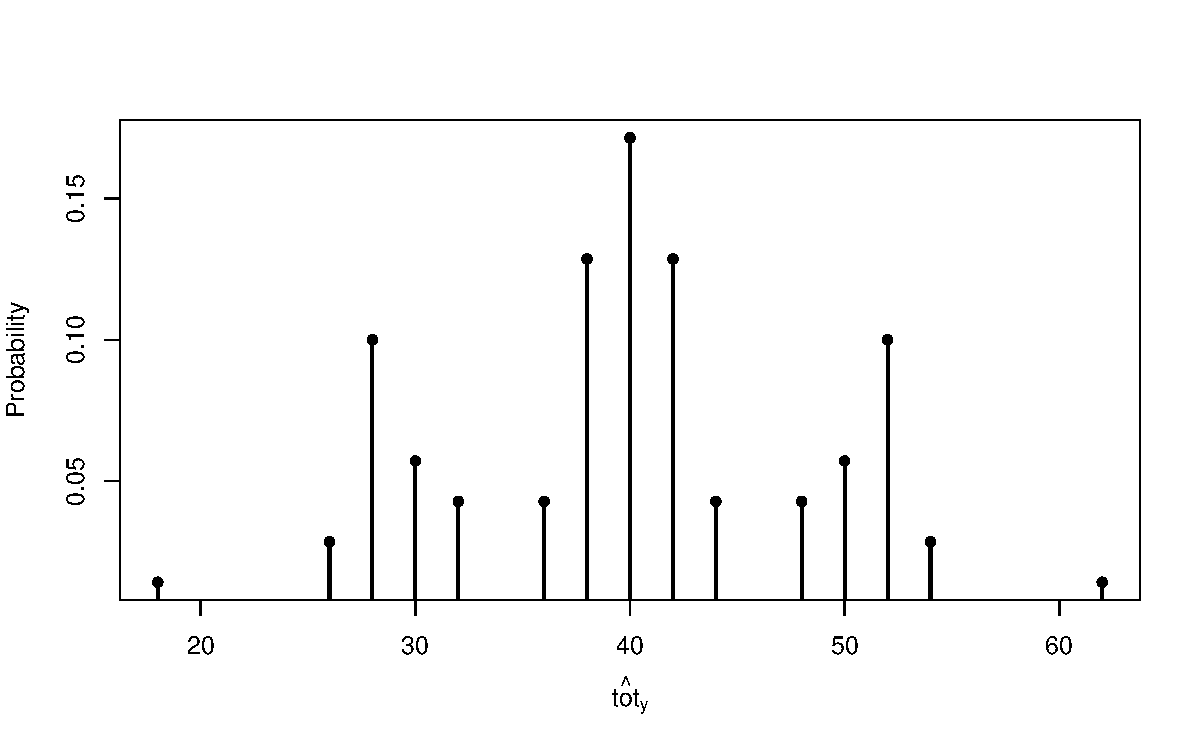
\includegraphics{problems/fig-distr}
            \caption{Sampling distribution of $\tys$}
            \label{fig:distribution}
        \end{figure}
    \end{Solution}

    %---------------------------------------------------------------------------
    \item Using the results from part a), compute numerically
        \begin{equation*}
            \EE(\,\tys) = \sum_{s \in \mathscr{S}_4} p(s) \, \tys(s)
        \end{equation*}
        and
        \begin{equation*}
            \var(\,\tys) = \sum_{s \in \mathscr{S}_4} p(s)
              \left\{\tys(s) - \EE(\tys)\right\}^2,
        \end{equation*}
        where $p(s) = 1/\binom{N}{n}$.

        \vspace{0.25em}

        Compare the numerical variance with the theoretical variance under
        simple random sampling without replacement:
        \begin{equation*}
            \var(\,\tys) = N^2\left(1 - \frac{n}{N}\right) \frac{\varyu}{n},
        \end{equation*}
        where
        \begin{equation*}
            \varyu = \frac{1}{N - 1}\sum_{i\in U}(y_i - \myu)^2.
        \end{equation*}

    \begin{Solution}
        Since all samples are equally likely,

\begin{Schunk}
\begin{Sinput}
> identical(mean(t_y), sum(y))
\end{Sinput}
\begin{Soutput}
[1] TRUE
\end{Soutput}
\end{Schunk}

        Hence $\EE(\,\tys) = \ty$: the estimator is unbiased.
        The variance obtained from the sampling distribution is

\begin{Schunk}
\begin{Sinput}
> mean((t_y - mean(t_y))^2)
\end{Sinput}
\begin{Soutput}
[1] 73.14286
\end{Soutput}
\end{Schunk}

        The theoretical variance of $\tys$ is

\begin{Schunk}
\begin{Sinput}
> sigma2_y <- var(y)
> N^2 * (1 - n / N) * sigma2_y / n
\end{Sinput}
\begin{Soutput}
[1] 73.14286
\end{Soutput}
\end{Schunk}

        The two values are identical.
    \end{Solution}
\end{Subtask}
\end{Problem}
